% Author: David Larsen <dcl9934@cs.rit.edu>
% Author: Doug Krofcheck <dpk3062@rit.edu>
\documentclass[11pt]{article}
\usepackage[margin=0.7in]{geometry}
\usepackage{listings}   %
\usepackage{needspace}  %
\usepackage{color}      %
\usepackage{ifthen}     % 
\usepackage{graphicx}   %
\usepackage{../includes/csc}        %
\usepackage{tikz}       %
\usetikzlibrary{shapes} %
\usepackage{tabularx}   % for helping matchtabular (matching questions)
\usepackage{textcomp}	% So our quotes in code don't look like shit
\usepackage{longtable}
\usepackage{multicol}
\usepackage[usenames,dvipsnames]{pstricks}
\usepackage{epsfig}
\setlength{\columnsep}{12em}

\lstset{ %
basicstyle=\footnotesize\ttfamily,       % the size of the fonts that are used for the code
numbers=left,                   % where to put the line-numbers
stepnumber=1,                   % the step between two line-numbers. If it's 1 each line will be numbered
numbersep=5pt,                  % how far the line-numbers are from the code
showspaces=false,               % show spaces adding particular underscores
showstringspaces=false,         % underline spaces within strings
tabsize=4,		                % sets default tabsize to 4 spaces
language=C,
upquote=true,
columns=fixed
}

\ifthenelse{\isundefined{\isAnswerKey}}
{
    \newenvironment{answer}{\large\lstset{basicstyle=\tiny\ttfamily}\color{white} \small{Answer:}}{}
}
{
    \newenvironment{answer}{\large\lstset{basicstyle=\large\ttfamily}\color{red} \small{Answer:}}{}
}

% ----- Start matchtabular definition -----
\newcounter{matchleft}
\newcounter{matchright}
\newenvironment{matchtabular}{%
  \setcounter{matchleft}{0}%
  \setcounter{matchright}{0}%
  \tabularx{\textwidth}{%
    >{\leavevmode\hbox to 1.5em{\stepcounter{matchleft}\arabic{matchleft}.}}X%
    >{\leavevmode\hbox to 1.5em{\stepcounter{matchright}\alph{matchright})}}X% 
    }%
}{\endtabularx}
% ----- End matchtabular definition -----

\title{CSCI-142 Exam 1 Review}
\author{Computer Science Community}
\date{\today}

\makeatletter
\let\thetitle\@title
\let\theauthor\@author
\let\thedate\@date
\makeatother

\begin{document}
\header
	\begin{enumerate}

\item Explain the relationship between machine language, assembly language, and high level languages.\\
\begin{answer}
\small{\textbf{Machine language} is a set of instructions that is executed directly as-is by the computer's CPU itself. This is considered the lowest level representation of a computer program, and, while it is possible to program directly in machine code, it is highly tedious and error prone, making higher level languages favorable. Writing machine code is typically only done when troubleshooting a system or when implementing extreme optimization.\\
\textbf{Assembly language} is also considered a low-level programming language, and, in particular, assembly usually has a near 1:1 relationship between the assembly code and the architechure's machine code instructions. Assembly languages are specific to a computer's architechture - for example, assembly code you write for your phone (almost certainly) wouldn't work on your laptop. An example of an assembly language is MIPS. Programming in assembly language (and lower) is commonplace in embedded systems work.
\\
Finally, \textbf{high level languages} are, in general, designed to be portable across many different architechtures. What separates the high level languages from their lower level counterparts is that, due to this fact, they require compiling, which translates your high-level code into a form which the machine can understand (which varies by architechture.) When people talk about programming languages, they are most often referencing one of the high level languages, unless otherwise specified. High level languages include C and C++, Python, and Java.}
\end{answer}




\item \textbf{Differences in Language Paradigms}

\begin{answer}
\end{answer}



\item \textbf{Programming Environments}

\begin{answer}
\end{answer}



\item \textbf{Modular Design and Development}

\begin{answer}
\end{answer}



\item List the 7 basic data types in C (not including the unsigned variants).

\begin{answer}
char, short, int, long, long long, float, double
\end{answer}



\item \textbf{Control Structures}

\begin{answer}
\end{answer}



\item \textbf{Operators}

\begin{answer}
\end{answer}



\item \textbf{Arrays}

\begin{answer}
\end{answer}



\item \textbf{I/O}

\begin{answer}
\end{answer}



\item What is the value of \texttt{i}?
\begin{verbatim}
#define THING1 40
#define THING2 32

#if THING1 < THING2
#define THING3 5
#elif THING2 < THING1
#define THING3 6
#else
#define THING3 7
#endif

int i = THING3;
\end{verbatim}
\begin{answer}
6
\end{answer}



\item \textbf{Memory and Program Layout}

Label the sections of the program in memory

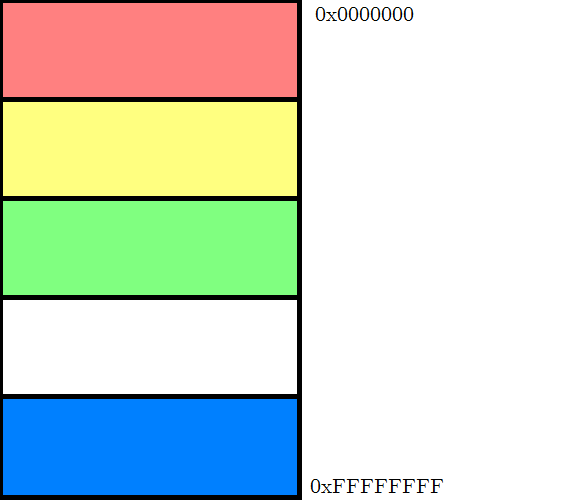
\includegraphics[width=50mm]{questions/programstructure.png}

\begin{answer}
red: text

yellow: data

green: heap

blue: stack
\end{answer}



\item \textbf{Functions}

\begin{answer}
\end{answer}



\item \textbf{Structs}

\begin{answer}
\end{answer}



\item \textbf{Strings}

\begin{answer}
\end{answer}



\item \textbf{Program Maintenance}

\begin{answer}
\end{answer}



\item \textbf{C Pointers}

\begin{answer}
\end{answer}



\item \textbf{Dynamic Storage}

\begin{answer}
\end{answer}




\end{enumerate}
\end{document}

Topics for this exam:
	- History and Evolution of Programming Languages
	- Differences in Language Paradigms
	- Programming Environments
	- Modular Design and Development
	- C: Variables, basic data types			DAKOTA/YAWAR
	- C: control structures, operators, arrays  YAWAR
	- C: basic I/O								YAWAR
	- C: basic CPP								DAKOTA
	- The OS: memory, program layout			DAKOTA
	- C: Functions, Structs, Strings			KATIE
	- Program Maintenance
	- C Pointers and Dynamic Storage			KATIE
